\pdfoutput=1
\documentclass[a4paper,12pt,titlepage, twoside]{article}
\usepackage[english]{babel}
\usepackage[utf8]{inputenc}
\usepackage{amssymb,amsmath}
\usepackage{algorithm,algpseudocode}
\usepackage[title,titletoc]{appendix}
\usepackage{natbib}
\usepackage{siunitx}
\usepackage{textcomp}
\usepackage[symbol]{footmisc}
\usepackage{booktabs}


\newcommand{\Author}{Zdeněk Rozsypálek}
\newcommand{\Title}{Active 3D mapping using laser range finder with steerable measuring rays}
\newcommand{\Acronym}{Acronym}
\newcommand{\WorkPackage}{WorkPackage}
\newcommand{\DocName}{Thesis}
\newcommand{\Subject}{\WorkPackage - \DocName}
\newcommand{\Keywords}{mobile robotics}
\newcommand{\Date}{1/1/2017}
\newcommand{\DOCVersion}{0.1}
\newcommand{\jed}[1]{\ensuremath{~\mathrm{#1}}} %příkaz pro sazbu fyzikálních jednotek

\def\clinks{false}

\usepackage{latexsym}
\usepackage{a4wide}
\usepackage{color} 
\usepackage{indentfirst}
\usepackage{graphicx}       %%% graphics for dvips
\usepackage{fancyhdr}
\usepackage{longtable}
\usepackage{pifont}
\usepackage{makeidx}
\usepackage{lastpage}
\usepackage{multirow}
\usepackage{dcolumn} 
\usepackage{epstopdf}
\usepackage{url}
\usepackage{listings}
\usepackage{caption}
\usepackage{subcaption}
\usepackage{relsize}
\usepackage{pdfpages}
\usepackage{url}

\lstset{breaklines=true,captionpos=b,frame=single,language=sh,float=h}
\lstloadlanguages{sh,c}
\def\lstlistingname{Listing}%{Výpis}
\def\lstlistlistingname{Listings}%{Seznam výpisů}

% European layout (no extra space after `.')
\frenchspacing

% no indent, free space between paragraphs
\setlength{\parindent}{1cm}
\setlength{\parskip}{1ex plus 0.5ex minus 0.2ex}

\usepackage{ifthen} %%% package for conditionals in TeX
\newread\testin
\def\softinput #1 {\let\next=\relax \openin\testin=#1
\ifeof\testin \message{Info: the file #1 does not exist}%
\else \closein\testin \def\next{\input #1 }\fi
\next}

\softinput{makeconfig}

\ifx\clinks\undefined
\def\clinks{true}
\fi

\ifx\pdfoutput\undefined %%% LATEX %%%
\def\nothtml{}  %%% \nothtml is defined if not processed with latex2html
%\usepackage[dvips]{graphicx}       %%% graphics for dvips
\usepackage[                %%% hyper-references for ps2pdf
bookmarks=true,%                   %%% generate bookmarks ...
breaklinks=true,%                  %%% breaks lines, but links are very small
hypertexnames=false,%              %%% needed for correct links to figures
colorlinks=\clinks,%
urlcolor=blue
]{hyperref}           %%% blue instead of cyan URLS
\hypersetup{
pdfcreator  = {LaTeX with hyperref package},
pdfproducer = {dvips + ps2pdf},
}
\else %%% PDFLATEX %%%
\def\nothtml{}  %%% \nothtml is defined if not processed with latex2html
%\usepackage[pdftex]{graphicx}        %%% graphics for pdfLaTeX
\usepackage[              %%% hyper-references for pdflatex
bookmarks=true,%                   %%% generate bookmarks ...
hypertexnames=false,%              %%% needed for correct links to figures
breaklinks=true,%                  %%% break links if exceeding a single line
colorlinks={\clinks},%
urlcolor=blue]{hyperref}           %%% blue instead of cyan URLS
\pdfadjustspacing=1                %%% force LaTeX-like character spacing
\fi

\hypersetup{  
pdfauthor={\Author},
pdftitle={\Title - \Acronym},
pdfsubject={\Subject},
pdfkeywords={\Keywords}
}

\def\BackgroundEPS#1#2#3#4{%
\special{ps: @beginspecial @setspecial initmatrix
0.1 setgray #2 #3 translate #4 dup scale}
\special{ps: plotfile #1}
\special{ps: @endspecial}
}

\pagestyle{fancy}
\setlength{\headheight}{18pt}
\renewcommand{\footrulewidth}{0.4pt}

%\lfoot{ČVUT FEL, Katedra Kybernetiky, Gerstner Laboratory}
\cfoot{}
%\rfoot{\thepage$/$\pageref{LastPage}}

\fancypagestyle{plain}

\fancyhead[R]{}

\newcommand{\DocBegin}{
\ifx\glreport\undefined
\else
\input{../common/glreport}
\fi
}


\renewcommand{\lstlistlistingname}{List of Algorithms}
\renewcommand{\lstlistingname}{Listing}
\definecolor{background_color}{rgb}{1.0, 1.0, 0.85}
\definecolor{comment_color}{rgb}{0.0, 0.5, 0.0}
\definecolor{keyword_color}{rgb}{0.0, 0.0, 1.0}
\definecolor{string_color}{rgb}{0.8, 0.0, 0.0}
\lstset{language=ksh}
\lstset{backgroundcolor=\color{background_color}}
\lstset{frameround=tttt}
\lstset{columns=fullflexible}
\lstset{keywordstyle=\color{keyword_color}\bfseries}
\lstset{commentstyle=\color{comment_color}}
\lstset{stringstyle=\color{string_color}}
\lstset{basicstyle=\ttfamily}
\lstset{showstringspaces=false}
\lstset{frame=single}
\lstset{keepspaces=true}
\lstset{tabsize=4}
\lstset{breaklines=true}
\lstset{captionpos=b}

\begin{document}
\DocBegin
%% Asymetric margins
%% LEAVE ONLY IN THE PRINTED VERSION
%% the electronic version should have symetric margins
% \setlength{\oddsidemargin}{+0.5cm} 
% \setlength{\evensidemargin}{-0.5cm}
%%

% Titulní stránka
\begin{titlepage}
\begin{center}

{\Large CZECH TECHNICAL UNIVERSITY IN PRAGUE}
\vskip 10pt

\vskip 8pt
{\Large Faculty of Electrical Engineering}
 
%\vskip 0pt plus 2fill
\vspace{50pt}
{\Huge\bf BACHELOR'S THESIS}\\
\vspace{40pt}

\includegraphics[width=10cm]{fig/lev.pdf}

\vspace{40pt}
{\Large\rm \Author } \\
\vspace{20pt}
{\Large\bf \Title}

\vspace{60pt}
{\bf Department of Control Engineering}\\
\vspace{5pt}   
{Thesis supervisor: {\bf Ing. Tomáš Petříček}}

\vspace{30pt}
%{\sc Prague 2013}
\end{center}
\end{titlepage}

\pagestyle{empty}
\cleardoublepage

%% The printed version of the acknowledgement page
%% LEAVE ONLY FOR PRINT
%~\vfill{}

\section*{Acknowledgements}

I would like to express my appreciation to Ing. Tomáš Petříček for his valuable and constructive suggestions during the planning and development of this thesis. I would also like to thank to the Department of Cybernetics of the Czech Technical University and Michal Němec for the provided hardware. Finally, I wish to thank my family for support throughout my study.

\vspace{2.5cm}

\newpage{}

%\cleardoublepage
%%

%% the scanned acknowledgement
%% LEAVE ONLY FOR THE ELECTRONIC VERSION
%~\vfill
%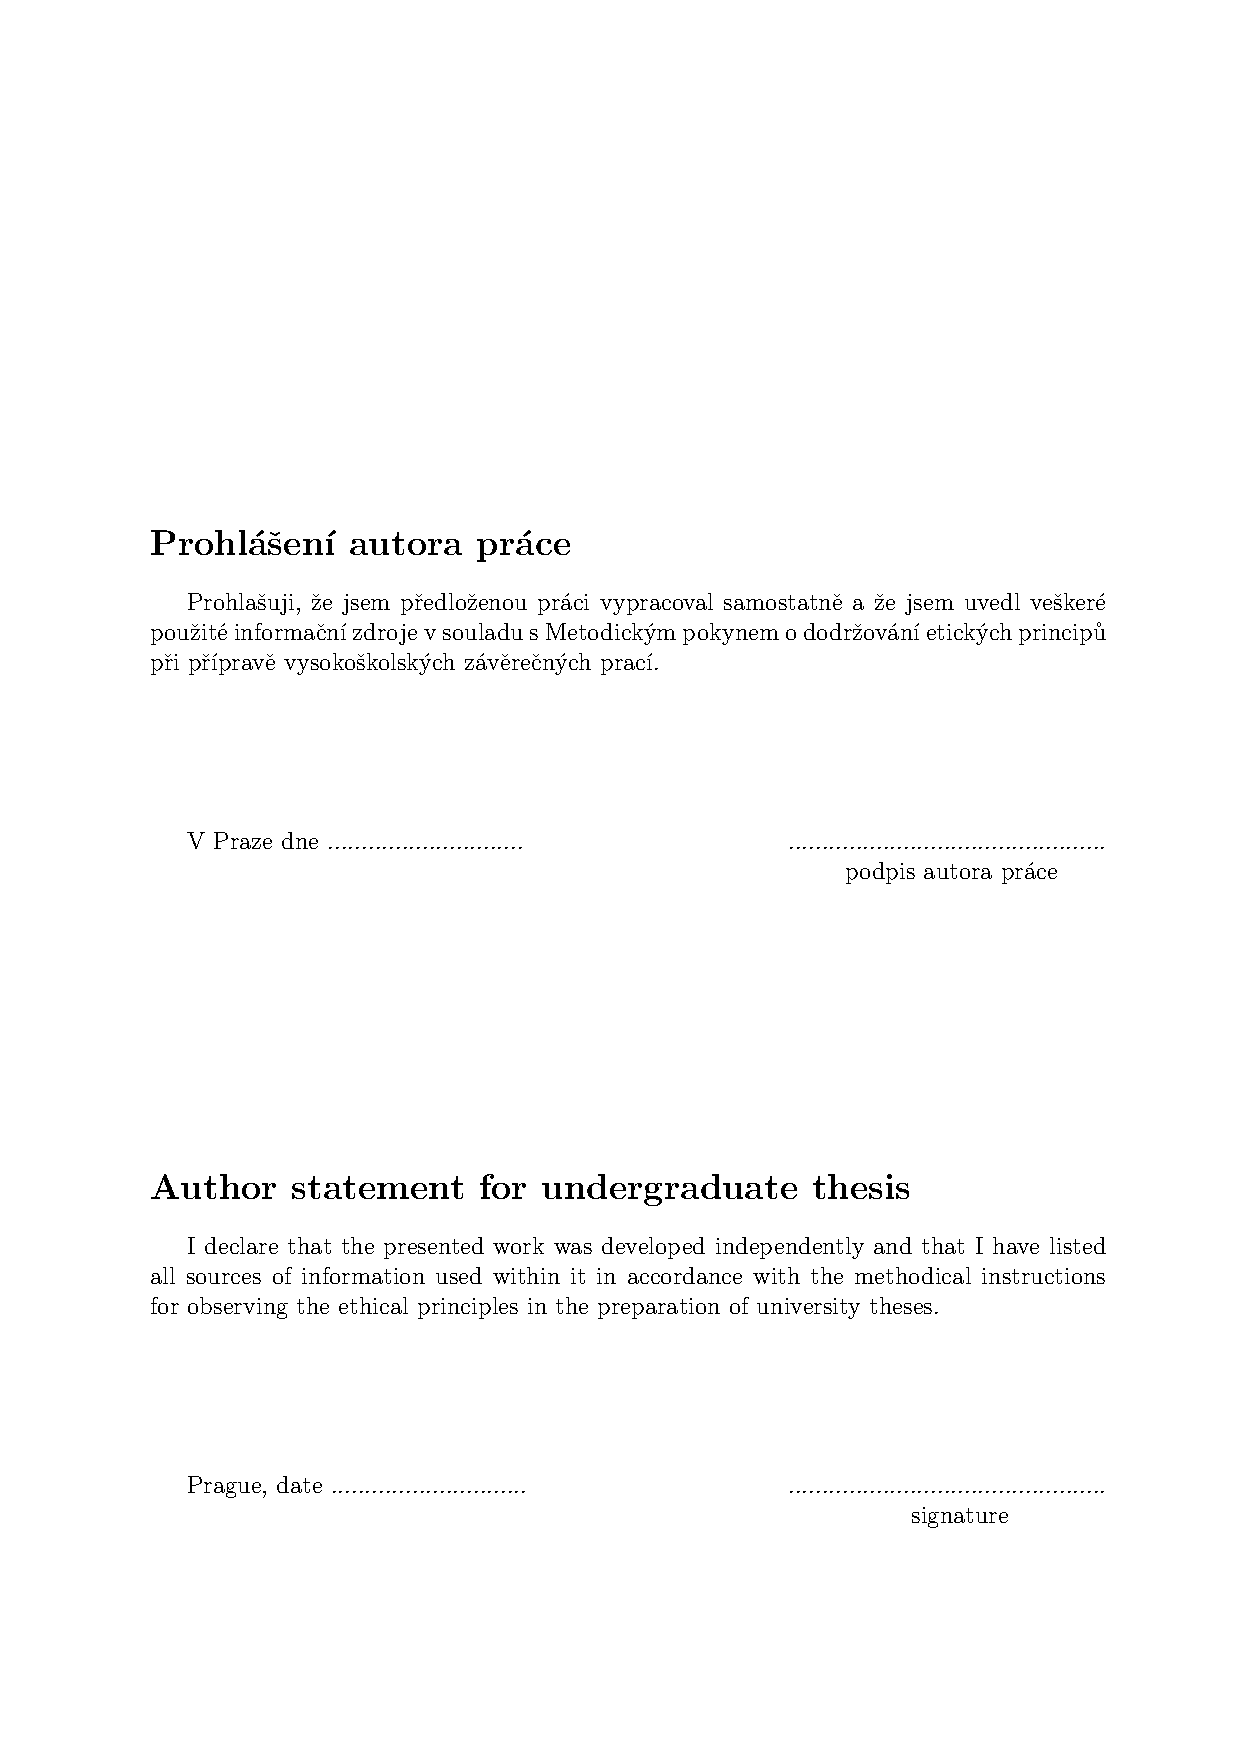
\includegraphics[width=1\textwidth]{acknowledgement.jpg}
%\cleardoublepage
%%

%% the scanned page (signed) with the assignement
%% LEAVE ONLY FOR THE ELECTRONIC VERSION
%\includepdf[pages={1}]{assignment_czech.pdf}
%\cleardoublepage
%\includepdf[pages={1}]{assignment_english.pdf}
%\cleardoublepage
%%

~\vfill{}

\section*{Acknowledgements}

I would like to express my appreciation to Ing. Tomáš Petříček for his valuable and constructive suggestions during the planning and development of this thesis. I would also like to thank to the Department of Cybernetics of the Czech Technical University and Michal Němec for the provided hardware. Finally, I wish to thank my family for support throughout my study.

\vspace{2.5cm}

\newpage{}

\cleardoublepage % it is prefered for the 1. level sections to start on the 

\vfill
\begin{center}
{\it \large Abstract}
\vspace{0.2cm}

\begin{minipage}{0.8\textwidth}{
The abstract in English. 
}
\end{minipage}
\end{center}
\vfill
\vspace{1cm}

\vfill
\begin{center}
{\it \large Abstrakt}
\vspace{0.2cm}

\begin{minipage}{0.8\textwidth}{
This Bachelor's thesis aims at control of the solid-state lidar sensor with a limited number of steerable rays. Besides planning of directions of the rays, the thesis is also devoted to creating dense 3D maps from sparse measurements. The thesis uses deep neural networks for planning the rays and reconstructing the dense maps. Planning part exploits the reinforcement learning concept for training of the neural network. An environment implementing a framework for training of reinforcement learning agents was created. The agent proposed in this thesis is using stochastic methods to achieve a sufficient scalability in the challenging environment.
\vspace{3mm}
\par \textbf{Keywords:} Lidar, reinforcement learning, deep neural network, 3D mapping, voxel map.
}
\end{minipage}
\end{center}
\vfill
\vspace{1cm}
\newpage{}

\cleardoublepage

\pagestyle{fancy}
\pagenumbering{roman}
\cfoot{\thepage}
\tableofcontents
\cleardoublepage

\pagestyle{fancy}
\pagenumbering{arabic}
\cfoot{}
\rfoot{\thepage$/$\pageref{LastPage}}
\setlength{\parskip}{0.35cm}

\lhead{INTRODUCTION}
\section{Introduction}

Lidar sensors offer an accurate distance measurements, which can be used for mapping srounding space. There is much utilization of volumetric space reconstructions in different fields. For example, lidar sensors are nowadays essential equipment for a large variety of autonomous vehicles. The sensor can help autonomous vehicles to orient itself in an environment. One of the most significant issues which prevent broader implementation of these sensors is a relatively high price. Breakthrough in this field is solid-state lidar. These lidars do not have moving parts, and their price should be circa hundreds of dollars \cite{quanergy2016}. Solid-state lidar can send limited number of rays in chosen directions per timestamp. Zimmermann et al. \cite{zimmermann2017} proposed mapping agent which creates dense reconstructions from sparse measurements. They also proposed prioritized greedy planning for choosing directions of these rays. The objective of this thesis is to apply reinforcement learning (RL) methods to learn planning of the rays and contribute to methods of controlling these sensors. RL is a field of study based on concepts of behavioral psychology, especially the trial and error method, and has in recent years experienced a rapid development due to the growth of computational power and neural networks improvement. Richard Sutton has made a helpful summary of RL concepts in his book \cite{sutton2012}. One of the biggest achievements was playing Atari games by a RL agent without any prior knowledge of the environment \cite{mnih2015}. Soon after was introduced an RL agent, able to solve simple continuous problems such as balancing inverse pendulum on a cart. Today state-of-the-art methods can solve complex problems with infinite action spaces. Although these methods reach great success, they still suffer from lack of sample efficiency - they need for training a lot of interactions with environment. This inefficiency makes creating agent controlling lidar very challenging, since training large neural networks is very time-consuming. The agent is divided into two parts - mapping and planning. The mapping part should create the best possible reconstruction from sparse measurements, while the planning part is focused on picking rays that will maximize reconstruction accuracy. Agents are trained using a publicly available dataset which contains drives of a car equipped with Velodyne lidar \cite{geiger2013}. Theoretical background of RL is discussed in first part of this thesis. In the second part are methods from first part used to solve the Lidar-gym environment \cite{rozsypalek2018}.
  
\clearpage

\lhead{THEORETICAL BACKGROUND}
\section{RL basics}
Firstly, environment where an agent is able to operate must be defined. Environment can be described as Markov decision process, where $S_t \in \mathcal{S}$ is a state from a set of possible states $\mathcal{S}$ in which environment is located in time $t$. Agent can usually observe the state of the environment and take action accordingly. Action is a probabilistic transition between states. Every action $A_t \in \mathcal{A}$ moves the environment from $S_t$ to $S_{t+1}$. The environment evaluates every action and returns appropriate reward $R_t$ (figure \ref{fig:rlconcept}). In RL set $\mathcal{A}$ is often called action space and set $\mathcal{S}$ observation space. The main goal of the agent is to find policy $\pi$ which maximises expected return. Return $G_t$ is a sum of discounted future rewards \cite{sutton2012}.
\begin{equation}
G_t = \sum\limits_{k=0}^{\infty}\gamma^k R_{t+k}
\end{equation}
where $\gamma \in [0,1]$ is discount factor. RL methods define how experiences from interacting with environment will change the policy.  Major issue is that maximising immediate reward is often not an effective approach to maximise expected sum of discounted rewards. This greedy policy can take the agent into very disadvantageous state. Thus, the agent must take into account future states and rewards. This is done by value function $V_pi(S_t)$ which assesses how advantageous is being in state $S_t$ with policy $\pi$.
\begin{equation}
V_\pi(S_t) \doteq  \mathbf{E}_\pi[G_t | S_t].
\end{equation}
Optimal policy $\pi^*$ is then defined as
\begin{equation}
\pi^*(S_t) \doteq \max\limits_\pi V_\pi(S_t),
\end{equation}
for all $S_t \in \mathcal{S}$.
In the past agents used big tables to estimate the value function. This is possible in environments with small action and observation spaces but is very memory consuming for larger environments and even impossible for continuous action or observation space. Therefore, modern methods use neural networks as function estimators.

\begin{figure}[!h]
\centering
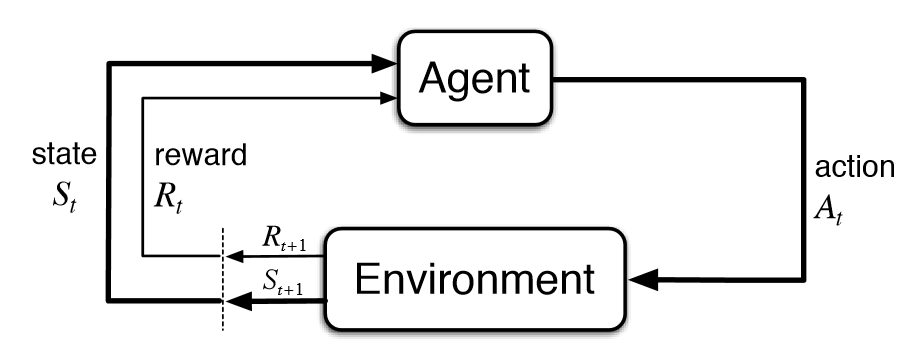
\includegraphics[scale=0.3]{fig/RL-concept.png}
\caption{RL concept}
\label{fig:rlconcept}
\end{figure}
\pagebreak

\subsection{Temporal difference learning}
Temporal difference (TD) learning combines the ideas of Monte Carlo methods and dynamic programming. It is able to learn directly from experience obtained by interactions with an environment without any prior knowledge of said environment. TD learning is done by following assignment in each timestamp \cite{sutton2012}
\begin{equation}
V(S_t) \gets V(S_t) + \lambda [R_{t} + \gamma V(S_{t+1}) - V(S_t)]
\end{equation}
where $\lambda \in \mathbb{R}^+$ is step size.

\subsection{Q-learning}
Q-learning is type of TD learning developed by Watkins \cite{watkins1992}. The state value $V$ from previous subsection is replaced by $Q$ value, which refers to quality of action in a particular state instead of quality of the state itself. When we rewrite TD learning (4) to Q-learning we get:
\begin{equation}
Q(S_t, A_t) \gets Q(S_t, A_t) + \lambda [R_{t} + \gamma \underset{A_{t+1}}{\max} Q(S_{t+1}, A_{t+1}) - Q(S_t, A_t)].
\end{equation}
Our policy here is to take action with maximal $Q$ value. That is called greedy policy. Obvious drawback of greedy policy is that it does not allow to explore the whole environment properly because an action with the highest $Q$ value is always chosen. A solution to this problem is sometimes take random action to explore the environment. This policy is often referred to as $\epsilon$-greedy policy.

\begin{algorithm}
\caption{$\epsilon$-greedy policy in pseudocode}
\begin{algorithmic}[1]
\Procedure{ChooseAction}{}
\State $\epsilon \gets \epsilon \cdot \epsilon_d$
\If {$\epsilon >$ random $\in (0,1)$}
\State action $\gets$ random $\in \mathcal{A}$
\Else 
\State action $\gets$ $\underset{A_t}{\max} Q(S_t, A_t)$
\EndIf
\State \Return action
\EndProcedure
\end{algorithmic}
\end{algorithm}

It is common to set $\epsilon = 1$ at the beginning of the training and decay rate $\epsilon_d$ close to one. General idea behind this policy assumes that it is needed to explore an environment first and then exploit agents experience.

\clearpage

\subsection{Prioritized experience replay}
Experience replay is biologically inspired mechanism introduced by Schaul et al. \cite{schaul2015} which stores all experiences (specifically: $S_t$, $A_t$, $R_{t}$, $S_{t+1}$) into a buffer and assigns priority to every experience. Main idea is that experiences with high TD should have higher priority. It is thus necessary to calculate priority $p$ from TD error:
\begin{equation}
p = (|\delta_t | + \eta)^\rho
\end{equation}
where $\rho$ indicates how much we prefer experiences with higher priority and $\eta \ll 1$ is a constant which helps to avoid priorities very close to zero. Considering a greedy selection would abandon experiences with low priority, a better approach is to choose experience $i \in \mathcal{I}$ with probability:
\begin{equation}
P(i) = \frac{p_i}{\sum_{j \in \mathcal{I}} p_j}
\end{equation}
where $\mathcal{I}$ is set of all experiences in the buffer. It is possible now to sample a batch of experiences for training using this probability. It removes correlation in the observation sequence and improves sample efficiency of DQN. It is feasible to store all experiences in a buffer sorted by priority but a more efficient implementation is a sum tree. That is a special case of binary tree, where value of each root is equal to the sum of its children values (see figure \ref{fig:sumtree}).
\vspace{5mm}
\begin{algorithm}
\caption{Retrieve node from sum tree in pseudocode}
\begin{algorithmic}[1]
\Procedure{GetChild(parent, value)}{}
\If {parent.left is None}
\State \Return parent
\EndIf
\If {value $\leq$ parent.left.value} 
\State \Return GetChild(parent.left, value)
\Else 
\State \Return GetChild(parent.right, value - parent.left.value)
\EndIf
\EndProcedure
\end{algorithmic}
\end{algorithm}
\clearpage
\begin{figure}[H]
\centering
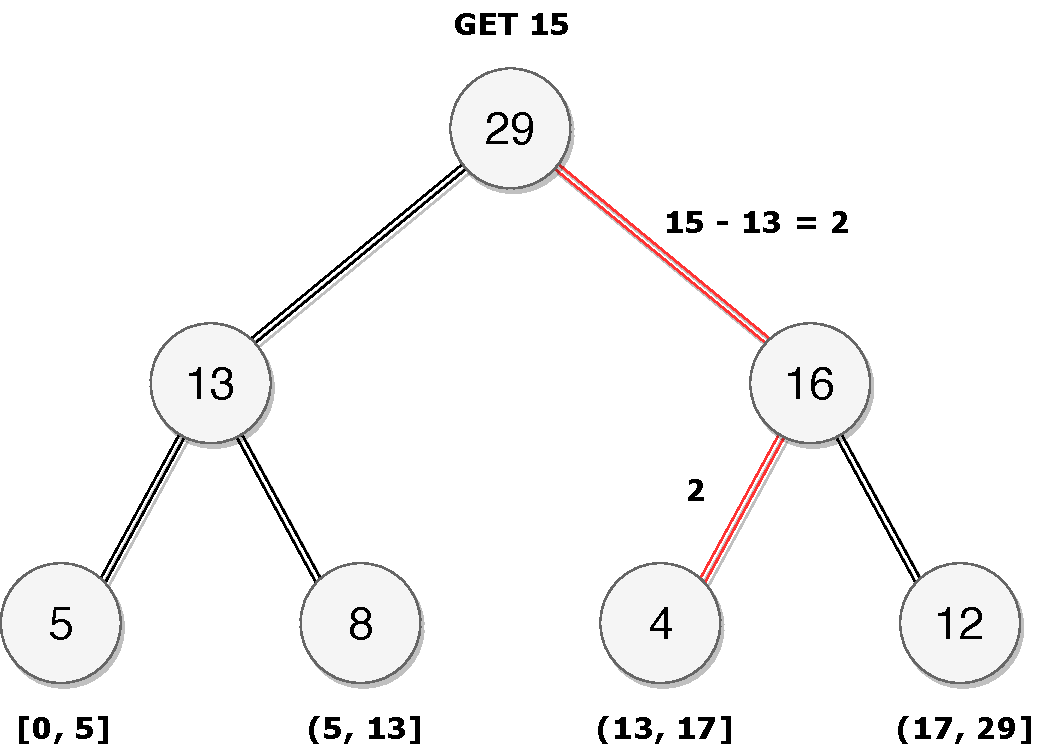
\includegraphics[scale=0.55]{fig/sumtree.pdf}
\caption{Sum tree example}
\label{fig:sumtree}
\end{figure}
\clearpage
\section{Deep neural networks in RL}
As was stated in previous chapter, tabular methods are very inefficient in large environments. In these instances is possible to use deep neural networks which can replace tables. Deep Q networks (DQN) proposed by Googles Deepmind \cite{mnih2015} outperformed all previous RL algorithms in playing Atari games. With neural networks grew also the popularity of policy gradient methods where function estimator outputs an action instead of Q values. Note that the most of these methods are general and not necessarily tied to neural networks.

\subsection{Deep Q network}
Neural network takes current state as input and outputs Q value for each possible action. Network is trained using gradients of Q value in current state with respect to trainable weights $\theta$ of our neural network.
\begin{align} \label{eq:qlearn}
\delta_t &= R_{t} + \gamma \underset{A_{t+1}}{\max}Q^\theta(S_{t+1}, A_{t+1}) - Q^\theta(S_t, A_t)\\
\theta_{t+1} &= \theta_t + \lambda \delta_t \nabla_\theta Q^\theta (S_t, A_t).
\end{align}
We are updating gradients in proportion to TD $\delta_t$. Unfortunately, this simple DQN agent suffers from a lack of sample efficiency and does not converge well. There are many techniques which can help DQNs to achieve satisfying results.

\subsection{Target network}
Target network is a technique which improves convergence of DQN learning \cite{mnih2015}. It uses two neural nets instead of one. The first is trained online network on a batch of data and the second target network is used for predictions during training. After the completion of training on a batch of data, the target network is updated
\begin{equation}
\theta^- = \tau \theta + (1-\tau)\theta^-
\end{equation}
where $\theta^-$ is set of trainable weights of the target network, $\theta$ indicates online network weights and $\tau \ll 1$ is constant.
TD $\delta$ is now calculated using target network:
\begin{equation}
\delta_t = R_{t} + \gamma \underset{A_{t+1}}{max}Q^{\theta^-}(S_{t+1}, A_{t+1}) - Q^\theta(S_t, A_t). 
\end{equation}
Target network stabilises training since predicting network does not change after each training step.

\subsection{Double Q-learning}
Classic Q-learning algorithm tends to overestimate actions under certain conditions. Hasselt et al. propose idea of Double Q-learning which decompose the max operation into action selection and action evaluation \cite{hasselt2015}. TD is then computed by following equation.
\begin{equation}
\delta = R_{t} + \gamma Q^{\theta^-}(S_{t+1}, \underset{A_{t+1}}{\text{argmax}}Q^\theta(S_{t+1}, A_{t+1})) - Q^\theta (S_t, A_t).
\end{equation}
Double DQN outperforms DQN in terms of value accuracy and in terms of policy quality.

\clearpage
\section{Policy gradient}
By this section the goal of neural network was predicting values on the basis of which we determined the policy. In policy gradient method neural network approximates the policy itself. 
\begin{equation}
\theta_{t+1} = \theta_t + \lambda \widehat{\nabla J(\theta_t)}
\end{equation}
where $J$ is performance measure with respect to our neural network parameters and $\widehat{\nabla J(\theta_t)}$ is stochastic estimate which approximates gradient of performance measure. In other words, this method is basically doing stochastic gradient ascent of $J$ with respect to $\theta$ \cite{sutton1999}. Policy gradient methods are outperforming DQNs especially in continuous action spaces, because their output is directly continuous action instead of Q-value for every possible action.

\subsection{Actor-Critic}
Thanks to predicting action directly, we gain possibility to predict in continuous action space, but the Q-value which assessed the quality of an action in certain state has been lost. That it why the Actor-Critic framework was created. It uses two separate neural networks - actor which predicts action and critic which assesses action advantage. Concept is visualised in the figure \ref{fig:actorcritic}.
\begin{figure}[H]
\centering
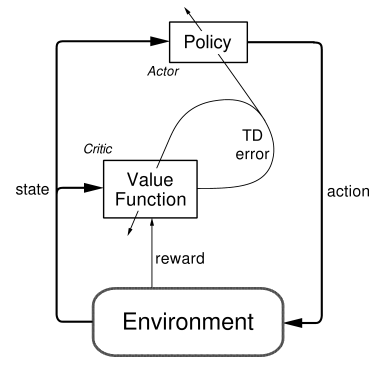
\includegraphics[scale=0.55]{fig/actor-critic.png}
\caption{Actor-Critic framework}
\label{fig:actorcritic}
\end{figure}
\clearpage

Consider critic using Q-values for update. $\theta$ and $\omega$ denote trainable weights of actor and critic, respectively. Critic update is similar to DQN:
\begin{align}
\delta_t &= r_t + \gamma Q^\omega(S_{t+1}, \mu ^\theta (S_{t+1})) - Q^\omega(S_t, A_t)\\
\omega_{t+1} &= \omega_t + \lambda \delta_t \nabla_\omega Q^\omega(S_t, A_t).
\end{align}
Note that instead of $A_{t+1}$ is now used function $\mu^\theta(S)$, which is an action estimate by actor neural network. Actor update rule is not so straightforward. 
\begin{equation}
\theta_{t+1} = \theta_t + \lambda\nabla_\theta \mu^\theta(S_t)\nabla_a Q^\omega (S_t, A_t)|_{a = \mu^\theta(S_t)}.
\end{equation}
This equation uses chain rule for derivatives to obtain gradient of Q-values with respect to trainable weights $\theta$. Namely:
\begin{equation}
\frac{\partial Q^\omega(S_t, A_t)}{\partial \theta} = \frac{\partial Q^\omega(S_t, A_t)}{\partial A_t} \frac{\partial A_t}{\partial \theta}.
\end{equation}
Actor neural network is updated by gradients which change action output to maximise Q-value of the critic \cite{silver2014}.
There are another approaches, which doesn't use Q-value as critic assessment, but they rather use so called advantage \cite{schulman2017}. These methods are beyond the scope of this thesis. 

\subsection{Stochastic Actor-Critic}
Stochastic Actor-Critic method is frequently used approach. In this method actor outputs parameters of a distribution and action itself is sampled within the parametrized distribution. It is standard to use normal distribution and predict the mean and variance of action. The biggest advantage of normal distribution is that it can be adjust to use of backpropagation \cite{hess2015}. Another benefit of stochastic actor is that it doesn't need any other techniques for action space exploration.

\subsubsection{Beta distribution}
On the other hand obvious drawback of normal distribution is that there is always some small probability to sample an outlier. There is also an issue for bounded action space. When mean value of normal distribution is close to the boundary, agent can experience not negligible bias. Solution for both problems is to use beta distribution as a stochastic policy \cite{chou17}. Beta distribution is defined by following function:
\begin{equation}
f(x;\alpha, \beta) = \frac{\Gamma(\alpha + \beta)}{\Gamma(\alpha)\Gamma(\beta)}x^{\alpha-1}(1-x)^{\beta-1},
\end{equation}
where $\alpha,\beta \in R^+_0$ are distribution parameters and $x \in [0, 1]$. $\Gamma$ is Euler's gamma function, which extends factorial into the set of real numbers. Beta distribution is shown in the figure \ref{fig:beta}.

\begin{figure}[H]
\centering
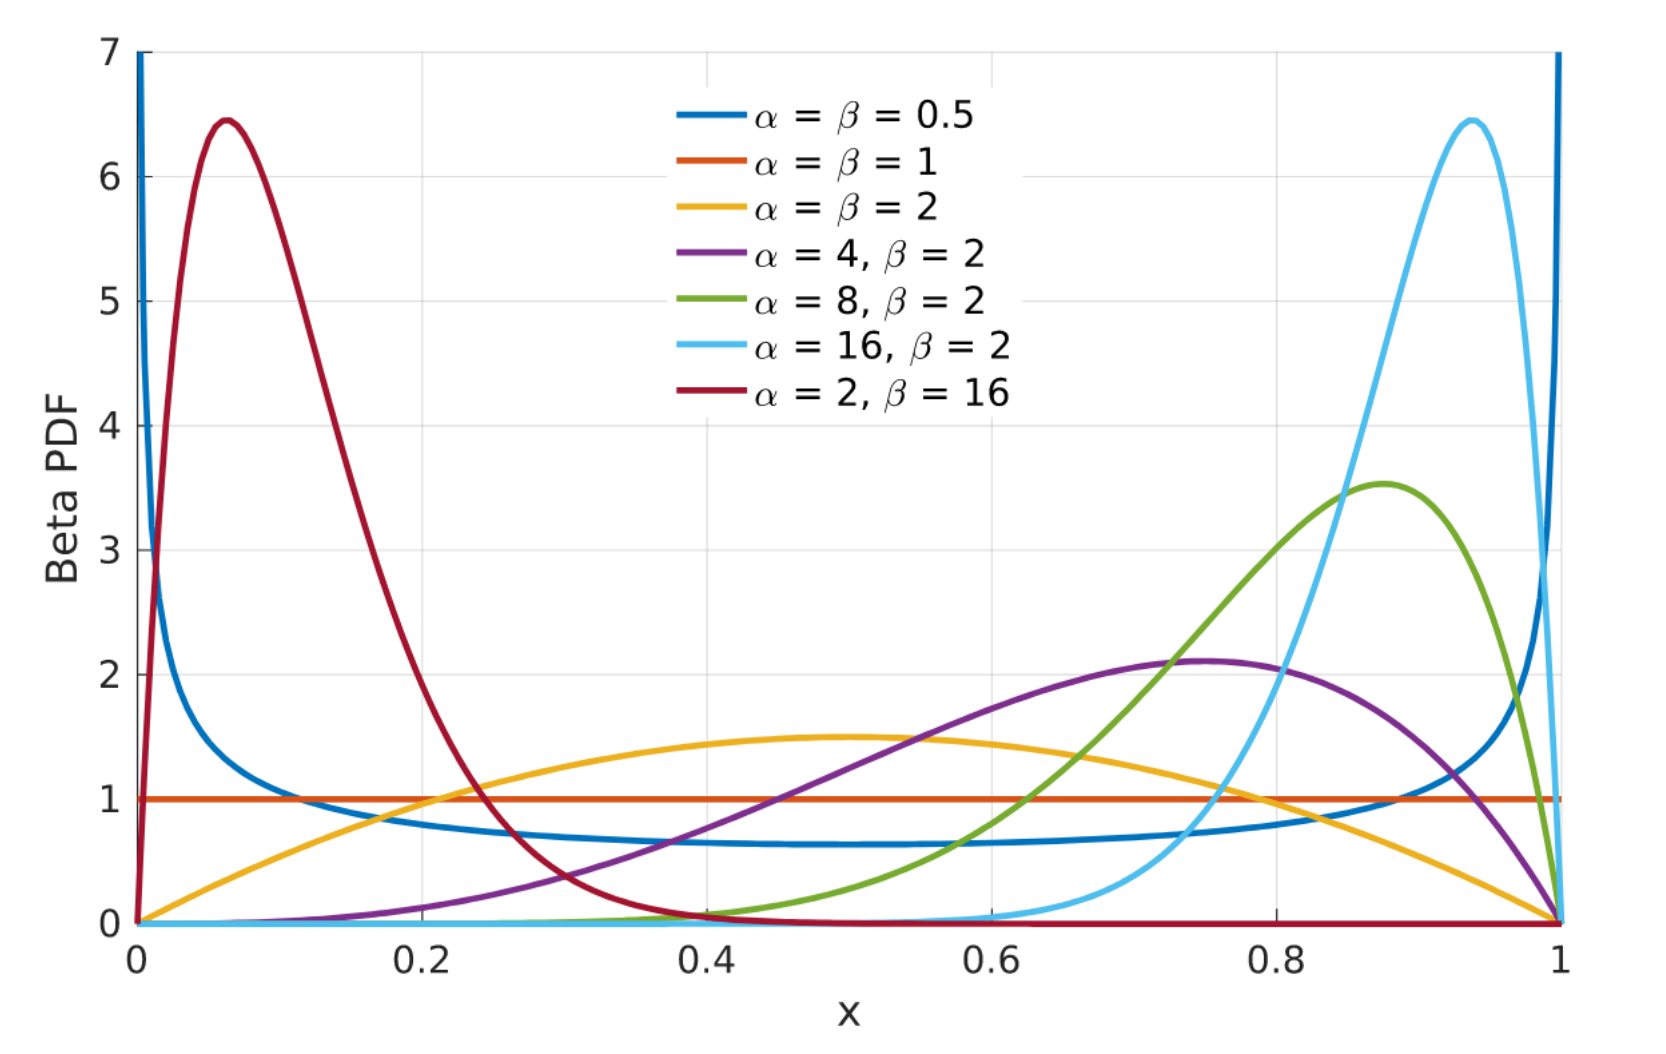
\includegraphics[scale=0.2]{fig/beta.png}
\caption{Probability density of beta distribution}
\label{fig:beta}
\end{figure}

For reinforcement learning is suitable only $\alpha, \beta \geq 1$. This makes beta distribution concave and unimodal. It can be ensured by using softplus activation and add one at the end of actor network.

\subsection{Deterministic policy gradients}
Deep deterministic policy gradient (DDPG) is one of methods exploiting the Actor-Critic framework. Whereas stochastic actor predicts distribution parameters and sample an action, DDPG outputs the action directly. Silver \cite{silver2014} has shown that deterministic policy can outperform its stochastic counterparts. Disadvantage of this approach is that it needs additional policy to ensure action space exploration. Exploration methods are discussed in subsection \ref{sec:exploration}.

\subsection{Wolpetinger policy}
Actor-Critic methods and DDPG work well in continuous action spaces, but there is a lot of usecases with large discrete action spaces, such as recommender systems or lidar planning. Wolpetinger policy is approach how to utilize continuous methods in discrete action space \cite{dulac2015}. Whole policy is illustrated in figure \ref{fig:wolpetinger}. Actor doesn't predict action directly, but it predicts so called proto-action $\tilde{A_t}$.
\begin{equation}
\tilde{A_t} = \mu^\theta(S_t).
\end{equation}
Proto action mostly isn't valid action $\tilde{A_t} \notin \mathcal{A}$. Thus it is necessary to find valid action corresponding to proto action. This is done by computing euclidean distance to every possible action.
\begin{equation} \label{eq:knn}
\mathcal{A}_{knn} = \overset{K}{\underset{a \in \mathcal{A}}{{\text{argmin}}}} | a - \tilde{A_t} |_2 .
\end{equation}
Usually policy choose $K$ closest actions to the proto action. $\mathcal{A}_{knn}$ is the set of closest action to the proto action. Whole set is then assessed by critic and action with highest Q-value is finally picked.
\begin{equation}
A_t = \underset{a \in \mathcal{A}_{knn}}{\text{argmax}} Q^\omega(S_t, a)
\end{equation}
\begin{figure}[!h]
\centering
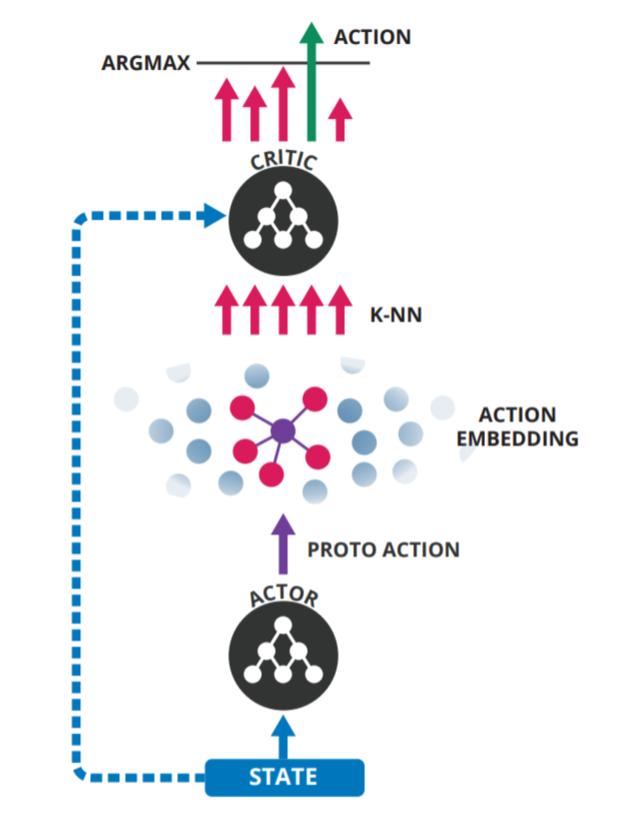
\includegraphics[scale=0.35]{fig/wolpetinger-policy.png}
\caption[Wolpetinger policy illustration] {Wolpetinger policy can be described in 3 steps. \textbf{1)} Actor outputs an action \textbf{2)} The $K$ nearest valid actions are found \textbf{3)} Choose the action which is assessed as the best by the critic}
\label{fig:wolpetinger}
\end{figure}

\subsection{Parameter and action space noise}
\label{sec:exploration}
In large action space is very important to emphasize agents exploration. Bad exploration can cause that agent converges prematurely and ends up in local optimum. DDPG commonly use stochastic policy to slightly modify actors actions.
\begin{equation} \label{eq:exploration}
\hat{A_t} = \mu^\theta(S_t) + \mathcal{N}(0, \sigma^2)
\end{equation}
where $\mathcal{N}$ is normal distribution with mean value equal to zero and variance, which is reducing during the training and $\hat{A_t}$ is perturbed action. Action space noise helps agent to explore the environment. \par Another approach is to apply noise directly to actors weights. It can sometimes lead to more consistent exploration and richer behaviours \cite{plappert2017}.
\begin{equation}
\hat{\theta} = \theta + \mathcal{N}(0, \sigma^2)
\end{equation}
where $\hat{\theta}$ is so called perturbed actor, which is interacting with environment. Major issue of parameter space noise is that it is much harder to tune. When we use action space noise it is easy to estimate its impact on actions (differences between both approaches can be seen in the figure \ref{fig:exploration}). Because of unpredictable influence of parameter space noise is necessary to use adaptive noise scaling.
\begin{align}
d &= |\hat{A_t} - \mu^\theta(S_t)|_2  \\
\sigma_{t+1} &= 
     \begin{cases}
       \kappa \sigma_t & \text{if } d \leq T \\
       \frac{1}{\kappa}\sigma_t & \text{otherwise}
     \end{cases}
\end{align}
where $\kappa$ is scaling factor slightly bigger than one and $T$ is threshold value, which has to be tuned to specific environment.
\par When is necessary to explore action space near to some specific action or include momentum of environment, it is possible to use Ornstein-Uhlenbeck random process \citep{lilicrap2015}. 
\begin{equation}
\hat{A_t} = \mu^\theta(S_t)  + \nu (\rho - \mu^\theta(S_t)) + \phi \mathcal{N}(0, 1),
\end{equation}
where $\nu, \phi \in [0, 1]$ are constants of the random process and $\nu$ is mean value around which we want to explore the action space. When $\nu = 0$ it is basic exploration as in expression \eqref{eq:exploration}.

\begin{figure}[H]
\centering
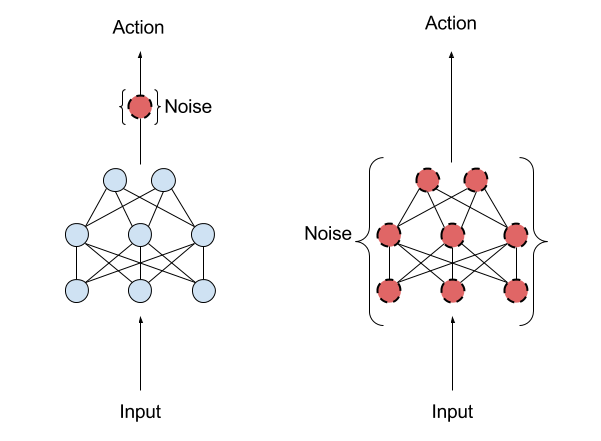
\includegraphics[scale=0.5]{fig/perturbations.png}
\caption{Left - action space noise, Right - parameter space noise}
\label{fig:exploration}
\end{figure}
\clearpage

\lhead{EXPERIMENT}
\section{Experiment}
Experiment aims at using reinforcement learning algorithms for solid-state lidar with steerable rays and limited number of rays. At first it was necessary to create environment where the agent can learn and evaluate \cite{rozsypalek2018}. Environment is written in python based on OpenAI gym interface \cite{openai2016}. It uses point clouds from Kitti dataset drives\cite{geiger2013}. One episode of learning in environment corresponds to one drive in Kitti dataset. Large point clouds from drives are processed into 3D voxel maps by C++ package \cite{petricek2017}, which also provides ray tracing engine for environment. Every voxel map is 3D array containing real numbers which corresponds to the occupancy $c$ of each voxel.
\begin{align}
\begin{split}
c &> 0 \quad \text{occupied voxel} \\
c &= 0 \quad \text{unknown occupancy} \\
c &< 0 \quad \text{empty voxel.}
\end{split}
\end{align}
Environment also offers visualisation of actions using Mayavi \cite{mayavi2011} and ASCII art. Agents use neural networks as function estimators, which are handled by Tensorflow \cite{tensorflow2015} and Keras \cite{keras2015}.

\subsection{Environments}
Lidar-gym implements several environments, which follow same template with different sizes. Observation space is local cutout of voxel map, which provides occupancies from sensor sparse measurements. Sensor is located in quarter of x axis and half of y and z axis of local cutout. Action space is divided into two parts. First part is dense voxel map reconstructed from observations (sparse measurements). Second part of action space are directions of measuring rays. Each ray has own azimuth and elevation. Environment expects directions in format of 2D array of booleans, where true means fired ray. Environments reward is negative logistic loss $-L$ \eqref{eq:loglos}. Lidar-gym defines environments with following parameters.

\begin{table}[h]
\centering
\begin{tabular}{|c||c|c|c|}
\hline
Name of environment     & Large                        & Small                        & Toy                       \\ \hline
Voxel map size [voxels] & 320 $\times$ 320 $\times$ 32 & 160 $\times$ 160 $\times$ 16 & 80 $\times$ 80 $\times$ 8 \\ \hline
Lidar FOV [\textdegree]           & 120 $\times$ 90              & 120 $\times$ 90              & 120 $\times$ 90           \\ \hline
Densitiy of rays        & 160 $\times$ 120             & 120 $\times$ 90              & 40 $\times$ 30            \\ \hline
Lidar range [m]         & 42                           & 42                           & 42                        \\ \hline
Number of rays          & 200                          & 50                           & 15                        \\ \hline
Voxel size [m] & 0.2 & 0.4 & 0.8 \\ \hline
Episode training time [min] & 120 & 15 & 1.5 \\ \hline
\end{tabular}
\caption{Environment description}
\end{table}

\clearpage
Due to the high time complexity were all experiments conducted in toy environment. RL agents need significantly more training steps than supervised agents. In OpenAI baselines \cite{openai2017} are RL agents trained for over million timestamps. One drive in Kitti dataset has on average 200 timestamps. All agents was trained and evaluated on different  drives from city part of dataset.

\subsection{Mapping agent}
Mapping agent is based on work of Zimmermann et al \cite{zimmermann2017}. It uses convolutional neural network (CNN) for reconstructing dense map from sparse measurements. 3D convolutional layers are used to learn the features and max pooling layers to avoid overfitting. Whole CNN architecture is described in figure \ref{fig:supervised}.
\vspace{3mm}
\begin{figure}[!h]
\centering
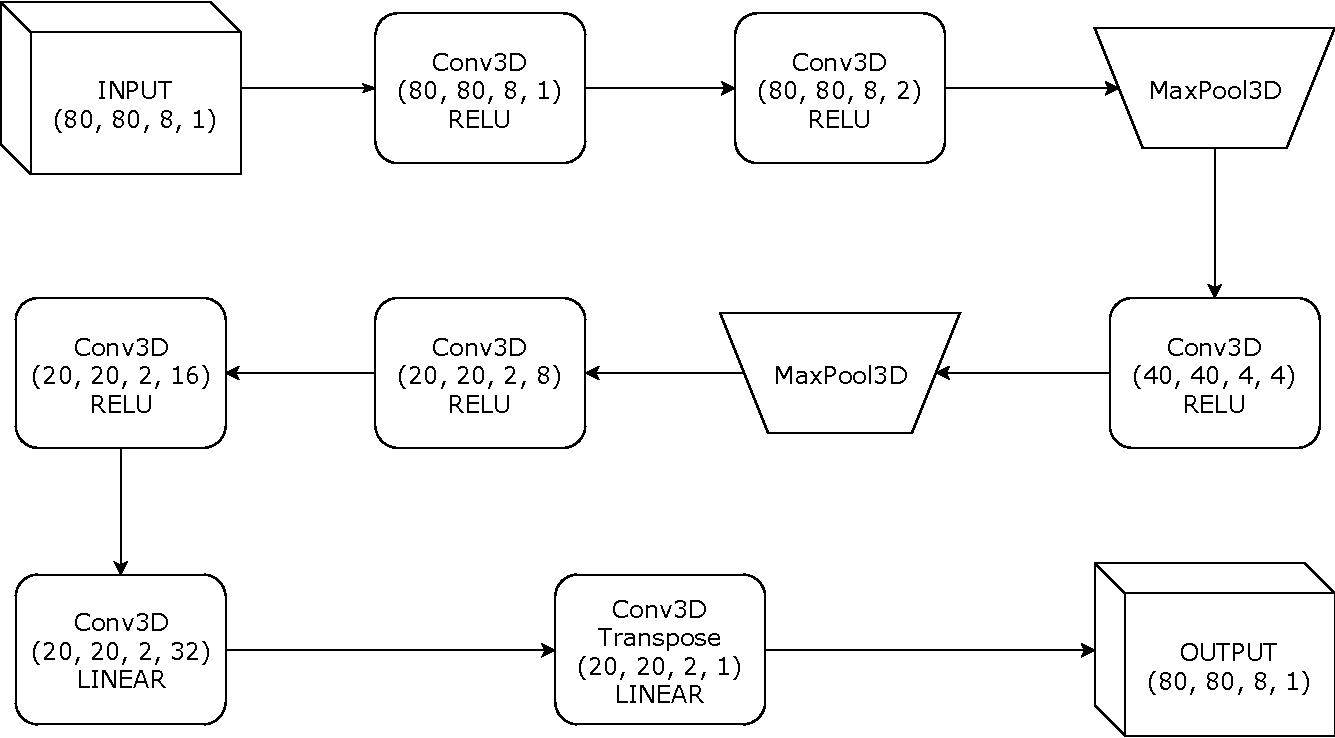
\includegraphics[scale=0.6]{fig/supervised.pdf}
\caption{Mapping network architecture}
\label{fig:supervised}
\end{figure}

For gradient descent is used logistic loss $L$ between ground truth map $Y$ and predicted dense map $\hat{Y}$.
\begin{equation} \label{eq:loglos}
L(Y, \hat{Y}) = \sum\limits_i w_i \log(1 + \exp(Y_i \hat{Y_i}))
\end{equation}
where $w$ are weights which balance importance of occupied and unoccupied voxels.
\clearpage
Unfortunately naive implementation of this loss function is computationally inconvenient and often cause numerical issues as underflow or overflow. To stabilize training following modified loss was used \cite{matconvnet2015}.
\begin{align} 
\begin{split}
a_i &= Y_i \hat{Y_i} \\
b_i &= \max(0, a_i) \\
L &= \sum\limits_i w_i (b_i + \log(\exp(-b_i) + \exp(a_i-b_i))).
\end{split}
\end{align}
At first we train mapping agent with random ray planning. Reconstructions of supervised agent are then used for training RL planning agents and after that is mapping agent retrained with RL agent picking the rays.
\subsection{Discrete planning agent}
Insomuch as environment input for direction of the rays is 2D binary array, first try is to use discrete agent. DQN is the most used option for discrete action space but in this use case it requires some tweaks. Note that number of possible actions is extremely large. Even in toy environment it is $40\times30 \choose 15$ $\approx 10^{34}$ of actions. Thus is necessary to emphasize on action space exploration. Further arises problem with $\epsilon$-greedy policy, because we are unable to process all possible actions and pick one with the biggest Q-value. To solve this issue is considered one ray as an action and for $K$ rays is TD from \eqref{eq:qlearn} now computed as:
\begin{align}
q(S_t, A_t) &= \max\limits_{A_t}^K Q^\theta(S_t, A_t)\\
\delta_t &= R_t + \gamma \overline{q}(S_{t+1}, A_{t+1}) - \overline{q}(S_t, A_t)
\end{align}
where $\overline{q}$ is average $Q$ value over $K$ actions with maximal $Q$ values.

\clearpage

\lhead{CONCLUSION}
\section{Conclusion}
First, we overviewed reinforcement learning concepts and described several methods which help convergence of the learning process. Then, we addressed the challenging multi-dimensional control task of selecting depth-measuring rays for 3D mapping. Various agents and model architectures were implemented and compared. All deterministic agents performed poorly in this specific task. The stochastic agent successfully outperformed the random planner. Action space size and time-complexity were two major blockers during the training. None of the trained RL agents can compete with the prioritized greedy planner proposed by Zimmermann et al. \cite{zimmermann2017}.


\subsection{Future work}
Experiment which would be worth conducting is an agents, which stands between simple and extended stochastic agent. The extended stochastic agent has action space consisting of 60 real numbers (15 rays with azimuth and elevation and for each alpha, beta parameters). That is very likely too much for network architecture used by agent. On the other hand, when only one distribution is outputted for all rays, it does not allow agent to create advanced policies. Solution could be to output for example three different distributions, each describing five rays. Another improvement could be achieved by adjusting neural network architecture. Especially splitting and merging layers of neural network, can have significant impact on performance. 

\cleardoublepage

% the list of all literature should be supplied in main.bib
\bibliographystyle{unsrt}
\bibliography{main}{}
\clearpage

\appendices
\lhead{\emph{APPENDIX \leftmark}} 
\section{CD Content}

In Table~\ref{tab:obsah} are listed names of all root directories on CD.

\vspace{1cm}
\begin{table}[!htb]
\centering
\begin{tabular}{lp{10cm}}
\textbf{Directory name} & \textbf{Description} \\

\hline
thesis & the thesis in pdf format \\
ctu\_thesis & latex source codes \\
lidar-gym & OpenAI gym environment \\
\hline
\end{tabular}
\caption{CD Content}
\label{tab:obsah}
\end{table}

\cleardoublepage

\section{List of abbreviations}\label{ape:abbreviations}

In Table \ref{table:abbreviations} are listed abbreviations used in this thesis.

\begin{table}[!htb]
\centering
\begin{tabular}{ll}
\textbf{Abbreviation} & \textbf{Meaning} \\
\hline
\textbf{CNN} & Convolutional neural network \\
\hline
\textbf{DDPG} & Deep deterministic policy gradients \\
\hline
\textbf{DQN} & Deep Q-learning \\
\hline
\textbf{MDP} & Markov decision process \\
\hline
\textbf{RL} & Reinforcement learning \\
\hline
\textbf{ReLu} & Rectified linear unit \\
\hline
\textbf{TD} & Temporal difference \\
\hline
\end{tabular}
\caption{Lists of abbreviations}
\label{table:abbreviations}
\end{table}
\cleardoublepage

\listoffigures
\cleardoublepage

\end{document}
